\documentclass[11pt,a4paper]{article}

% SIH26169 Technical Report (separate from beamlock_technical_deep_dive.tex)
\usepackage[margin=0.85in]{geometry}
\usepackage{amsmath,amssymb,bm}
\usepackage{booktabs}
\usepackage{array}
\usepackage{graphicx}
\usepackage{xcolor}
\usepackage{hyperref}
\usepackage{enumitem}
\usepackage{caption}
\usepackage{subcaption}
\usepackage{titlesec}
\usepackage{fancyhdr}
\usepackage{setspace}
\usepackage{listings}
\usepackage{float}
\usepackage{multirow}
\usepackage{longtable}

\definecolor{BeamTeal}{HTML}{1F6F8B}
\definecolor{BeamInk}{HTML}{162436}
\definecolor{BeamMuted}{HTML}{5F6E82}
\definecolor{CodeBg}{HTML}{F4F7FA}
\definecolor{DoneGreen}{HTML}{1B7F4E}
\definecolor{ExtraBlue}{HTML}{1F6F8B}

\newcommand{\Done}{\textcolor{DoneGreen}{\textbf{Done}}}
\newcommand{\Extra}{\textcolor{ExtraBlue}{\textbf{Beyond PS}}}
\newcommand{\Partial}{\textcolor{orange}{\textbf{Partial}}}

\hypersetup{
  colorlinks=true,
  linkcolor=BeamTeal,
  urlcolor=BeamTeal,
  citecolor=BeamInk
}

\captionsetup{font=small,labelfont=bf,skip=5pt}
\titleformat{\section}{\large\bfseries\color{BeamInk}}{\thesection}{0.8em}{}
\titleformat{\subsection}{\normalsize\bfseries\color{BeamTeal}}{\thesubsection}{0.7em}{}
\titleformat{\subsubsection}{\normalsize\itshape\color{BeamInk}}{\thesubsubsection}{0.6em}{}

\pagestyle{fancy}
\fancyhf{}
\fancyhead[L]{\small\color{BeamMuted}BeamLock --- SIH Technical Report}
\fancyhead[R]{\small\color{BeamMuted}SIH26169}
\fancyfoot[C]{\thepage}
\renewcommand{\headrulewidth}{0.4pt}

\graphicspath{{figures/}}
\setstretch{1.22}
\setlist[itemize]{leftmargin=1.4em,itemsep=0.12em}
\setlist[enumerate]{leftmargin=1.4em,itemsep=0.12em}

\lstset{
  basicstyle=\ttfamily\small,
  backgroundcolor=\color{CodeBg},
  frame=single,
  rulecolor=\color{BeamMuted},
  breaklines=true,
  columns=fullflexible
}

\begin{document}

% ---------- TITLE PAGE ----------
\begin{titlepage}
\centering
\vspace*{0.8cm}
{\color{BeamMuted}\large Smart India Hackathon 2026}\\[0.35cm]
{\color{BeamTeal}\Large Technical Report}\\[0.9cm]
{\rule{\textwidth}{1.2pt}}\\[0.45cm]
{\LARGE\bfseries\color{BeamInk} BeamLock}\\[0.3cm]
{\large AI-Based Virtual Camera Tracking System for\\
Coarse Alignment of Mobile Free-Space Optical\\
Communication (FSOC) Terminals}\\[0.45cm]
{\rule{\textwidth}{1.2pt}}\\[1.0cm]

\begin{minipage}{0.88\textwidth}
\raggedright
\textbf{Problem Statement ID:} SIH26169\\[0.2cm]
\textbf{Organization:} Department of Space / ISRO\\[0.2cm]
\textbf{Theme:} Smart Automation / Space Technology\\[0.2cm]
\textbf{Category:} Software\\[0.2cm]
\textbf{Team Name:} Cadets\\[0.2cm]
\textbf{Repository:} \url{https://github.com/MudithDShetty/SIH}\\[0.2cm]
\textbf{Software package:} \texttt{fsoc-virtual-tracker} (product name: BeamLock)
\end{minipage}

\vfill
{\large Version 1.2 --- \today}\\[0.45cm]
{\small\textit{Physics-informed PAT sandbox for algorithm development and SIH evaluation.\\
Not a certified BER model or flight-qualified optical terminal.}}
\end{titlepage}

\begin{abstract}
\noindent
This report documents \textbf{BeamLock}, an AI-assisted virtual camera tracking system developed for SIH26169.
The software closes a real-time coarse pointing--acquisition--tracking (PAT) loop inside a configurable virtual scene: moving optical beacons, an azimuth/elevation (AZ/EL) virtual camera plant with rate limits, Classical and hybrid AI detectors, constant-velocity Kalman tracking, covariance-scaled raster re-acquisition, disturbance injection, and automated performance logging.
\textbf{Section~\ref{sec:compliance} explicitly traces every SIH26169 expected-solution prerequisite, Parameters-table item, evaluation path, and submission deliverable to implemented evidence}, and additionally lists beyond-PS capabilities (physics channel, Link Readiness Fine handoff, Monte Carlo, dual Physics/PS profiles).
Verified matched-seed Classical vs AI results, acquisition Monte Carlo against an ESTOL-inspired $60\,\mathrm{s}$ bound, and representative HUD captures are reported with honest limitations (notably slew-lag-limited mean pixel error in the physics closed loop).
\end{abstract}

\tableofcontents
\newpage

%% ============================================================
\section{Problem Understanding}
%% ============================================================

\subsection{Operational context}
Free-Space Optical Communication (FSOC) can deliver gigabit-to-terabit class links using narrow laser beams in unlicensed spectrum with high immunity to radio-frequency interference.
On mobile platforms (UAVs, aircraft, LEO terminals), the beam must remain aligned through a PAT process that typically comprises:
\begin{enumerate}
  \item \textbf{Coarse alignment:} locate the remote beacon and keep it inside the acquisition camera field of view (FOV);
  \item \textbf{Fine alignment:} null residual pointing error with a high-bandwidth mechanism (e.g.\ fast steering mirror / FSM and four-quadrant detector / 4-QD) before communications beam lock.
\end{enumerate}
Hardware PAT benches require costly cameras, gimbals, and optics, which slows algorithm iteration.
SIH26169 therefore asks for a \textbf{software virtual camera} in which coarse alignment algorithms can be developed, disturbed, measured, and compared---including AI assistance---without specialized hardware.

\subsection{Official problem decomposition}
Before fine pointing can engage, coarse alignment must:
\begin{itemize}
  \item observe the environment through a virtual camera viewport;
  \item acquire and detect the remote beacon under clutter and noise;
  \item estimate beacon position and motion;
  \item continuously reposition the camera (pan--tilt class AZ/EL control).
\end{itemize}
The SIH Parameters table further specifies suggested screen/camera sizes, FOV, motion classes (including figure-of-eight), named noise and weather grades, and performance targets (acquisition time, tracking error, lock retention, FPS).
The Evaluation table weights live demonstration, Benchmark Performance-1 (scenario logs), Benchmark Performance-2 (judge MP4 at $\sim$30\,fps with PTZ bypass), and technical Q\&A.
Full prerequisite-by-prerequisite compliance is tabulated in Section~\ref{sec:compliance}.

\subsection{Scope and non-goals}
BeamLock is a real-time PAT \emph{sandbox} ($\sim$60\,fps class on a laptop).
It is \textbf{not} a certified bit-error-rate (BER) / outage calculator, split-step phase-screen wave-optics propagator, or flight-qualified optical terminal software.
Physics models follow Andrews \& Phillips order-of-magnitude horizontal / UAV-class path intuition and are calibrated for demo dynamics, not flight certification.

%% ============================================================
\section{SIH Prerequisites and Compliance Traceability}
\label{sec:compliance}
%% ============================================================

\noindent\textbf{Statement of compliance.}
Team Cadets implemented \textbf{all mandatory expected-solution prerequisites} of SIH26169, aligned the software to the official Parameters table via a dedicated PS profile, prepared the Evaluation Stage~1/2 tooling (including Benchmark-2 PTZ bypass), and submitted the required documentation deliverables.
In addition, BeamLock ships capabilities \textbf{beyond} the written problem statement (physics channel, Fine handoff mock, Monte Carlo acquisition, hybrid fusion, Link Readiness).
Tables~\ref{tab:prereq}--\ref{tab:beyond} are the judge-facing evidence maps.

\subsection{Expected solution prerequisites (mandatory)}
\begin{table}[H]
\centering
\caption{SIH26169 expected-solution prerequisites vs BeamLock evidence}
\label{tab:prereq}
\footnotesize
\begin{tabular}{@{}p{4.5cm}c p{7.6cm}@{}}
\toprule
\textbf{PS prerequisite} & \textbf{Status} & \textbf{Evidence in software / docs} \\
\midrule
Configurable virtual environment & \Done & Sliders + Calm/UAV/Stress presets (\texttt{ui/}) \\
One or more moving targets/beacons & \Done & 1/2 beacons (\texttt{B}); multi-spot association \\
Movable virtual camera (pan/tilt) & \Done & AZ/EL plant, rate/accel limits (\texttt{scene/camera.py}) \\
Automatic beacon detection & \Done & Classical + YOLO + Hybrid (\texttt{detector/}) \\
Continuous CV tracking & \Done & Constant-velocity Kalman state machine \\
Closed-loop camera repositioning & \Done & Drive from Kalman estimate (not ground truth) \\
Disturbances (turb./vib./noise) & \Done & Cn$^2$ channel + vibration + selectable noise \\
Real-time performance display & \Done & HUD: µrad error, lock, readiness, FPS \\
AI-assisted tracking & \Done & Trained YOLOv8n + live hybrid fusion path \\
Classical vs AI comparison & \Done & \path{scripts/run_comparison.py} matched-seed matrix \\
Automatic performance logs & \Done & CSV + run-sheet JSON + Streamlit/PDF \\
Re-acquisition after lock loss & \Done & Raster search (default); spiral available in code \\
\bottomrule
\end{tabular}
\end{table}

\subsection{Parameters table (PS profile + both modes)}
\begin{table}[H]
\centering
\caption{Official Parameters / Specifications coverage}
\label{tab:paramsfull}
\footnotesize
\begin{tabular}{@{}p{3.5cm}p{4.0cm}p{5.2cm}@{}}
\toprule
\textbf{Parameter} & \textbf{PS suggestion} & \textbf{BeamLock status} \\
\midrule
Screen size & $\ge 2000\times2000$ & \Done\ via \texttt{--profile ps} \\
Camera resolution & $640\times480$ & \Done\ PS profile \\
Camera FOV & $4^\circ\times3^\circ$ & \Done\ PS; Physics keeps 2.5\,mrad class \\
Beacon appearance & $\sim10\times10$ class & \Done\ square beacon in PS profile \\
Motions ($\ge4$) & Incl.\ figure-of-eight & \Done\ linear, circular, random, Fig-8 \\
Slew rate & $\sim5^\circ/\mathrm{s}$ class & \Done\ PS profile slew \\
Noise types & Gaussian, S\&P, Poisson & \Done\ cycle with \texttt{N} \\
Weather / atmosphere & Clear--Low light & \Done\ presets with \texttt{M} \\
Tracking error guidance & $\le10$\,px & \Done\ offline B2 $\sim$0.8\,px; PS path for closed-loop \\
Acquisition time & Short / ESTOL-class & \Done\ MC median $<1$\,s (Table~\ref{tab:mc}) \\
Lock retention logging & Required & \Done\ \% in CSV/JSON/HUD \\
FPS / latency logging & Required & \Done\ session metrics + HUD \\
\bottomrule
\end{tabular}
\end{table}

\subsection{Evaluation, deliverables, and extras}
Tables~\ref{tab:evaldeliver} and~\ref{tab:beyond} complete the compliance picture.

\begin{table}[H]
\centering
\caption{Evaluation layers and submission deliverables}
\label{tab:evaldeliver}
\footnotesize
\begin{tabular}{@{}p{4.2cm}c p{7.8cm}@{}}
\toprule
\textbf{Item} & \textbf{Status} & \textbf{Evidence} \\
\midrule
\multicolumn{3}{@{}l}{\textit{Evaluation}} \\
Functional live demo & \Done & Full GUI closed loop; demo checklist \\
Benchmark Performance-1 & \Done & Scenario runs $\rightarrow$ CSV/JSON logs \\
Benchmark Performance-2 & \Done & \path{scripts/benchmark_video.py} PTZ bypass \\
Architecture / AI / docs & \Done & This report + \path{docs/user_manual.md} \\
\midrule
\multicolumn{3}{@{}l}{\textit{Deliverables}} \\
Working software + source & \Done & \texttt{python main.py}; package tree \\
Technical report (10--15\,pp) & \Done & This PDF \\
User manual & \Done & \path{docs/user_manual.md} \\
Automatic performance logs & \Done & CSV, JSON, Streamlit PDF \\
Standalone packaging path & \Done & \path{scripts/build_exe.py} \\
Demo video & \Partial & Demo MP4 present ($\sim$53\,s; optional 3--5\,min) \\
\bottomrule
\end{tabular}
\end{table}

\subsection{Beyond the written problem statement}
\begin{table}[H]
\centering
\caption{Additional capabilities beyond PS minima}
\label{tab:beyond}
\footnotesize
\begin{tabular}{@{}p{5.2cm}c p{6.9cm}@{}}
\toprule
\textbf{Extra capability} & \textbf{Tag} & \textbf{Module / evidence} \\
\midrule
Cn$^2\rightarrow r_0$ atmospheric channel & \Extra & \path{physics/atmosphere.py} \\
Gaussian link budget + SNR & \Extra & \path{physics/link_budget.py} \\
Link Readiness score $S\in[0,1]$ & \Extra & \path{metrics/link_readiness.py} \\
Coarse$\rightarrow$Fine 4-QD/FSM mock & \Extra & \path{control/fine_pointing.py} \\
Hybrid AI+classical fusion & \Extra & \path{detector/hybrid_detector.py} \\
Dual Physics / PS profiles & \Extra & \path{profiles.py} \\
Acquisition Monte Carlo vs 60\,s & \Extra & \path{scripts/monte_carlo_acquisition.py} \\
Clutter Pd/Pfa + ablation + demo tools & \Extra & \texttt{scripts/evaluate\_detection.py} et al. \\
\bottomrule
\end{tabular}
\end{table}

\noindent\textbf{Compliance summary.}
Mandatory PAT prerequisites: \textbf{complete}.
Parameters table: \textbf{covered} (PS profile + shared controls).
Evaluation Stages~1--2 tooling: \textbf{ready}.
Deliverables: \textbf{complete} (demo video present; optional lengthening is the only partial item).
Beyond-PS scientific PAT features: \textbf{implemented and demonstrated}.

%% ============================================================
\section{System Architecture}
%% ============================================================

\subsection{Closed-loop overview}
Figure~\ref{fig:arch} shows the end-to-end architecture.
Operator configuration drives a virtual world; disturbances and link physics degrade the camera view; detection and tracking produce camera drive commands on a control bus; outputs provide live HUD metrics and archival logs.
A feedback path returns AZ/EL drive (coarse, re-acquisition, or fine mock) to the virtual camera plant.

\begin{figure}[H]
\centering
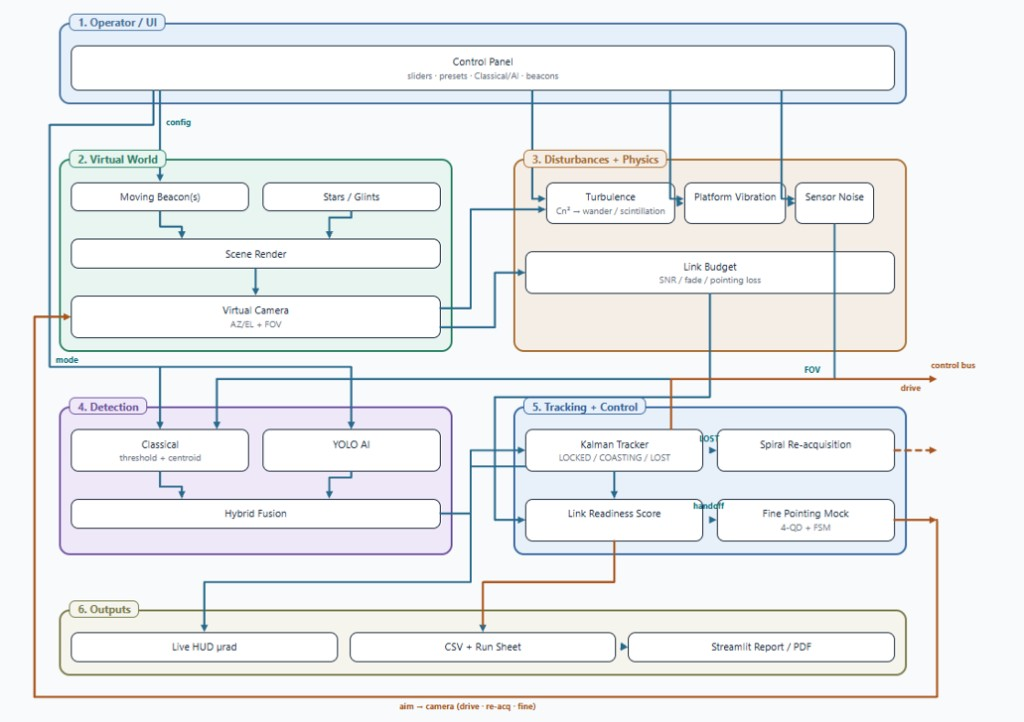
\includegraphics[width=0.95\textwidth]{architecture_diagram.png}
\caption{BeamLock real-time PAT architecture.
Forward path: scene $\rightarrow$ disturbances/physics $\rightarrow$ detection $\rightarrow$ tracking/control $\rightarrow$ outputs.
Feedback path: Kalman / re-acquisition / fine mock drives the virtual camera AZ/EL plant.
(\emph{Note:} the live default re-acquisition pattern is \textbf{raster}; spiral generation remains in code for literature comparison.)}
\label{fig:arch}
\end{figure}

\subsection{Per-frame control law}
Each simulation frame executes:
\begin{enumerate}
  \item Advance beacon kinematics and render scene (with clutter if enabled).
  \item Apply atmospheric wander/scintillation appearance coupling, platform vibration, and sensor noise to the FOV crop.
  \item Compute link budget quantities ($P_{rx}$, SNR, pointing loss) and Link Readiness $S\in[0,1]$.
  \item Detect beacon(s) via Classical \emph{or} Hybrid AI path (mutually exclusive live mode).
  \item Update Kalman tracker; emit state \texttt{LOCKED} / \texttt{COASTING} / \texttt{LOST}.
  \item Select plant command:
  \begin{itemize}
    \item if \texttt{LOST}: raster re-acquisition waypoints with distance-scaled slew;
    \item else if Fine stage active: mock 4-QD residual nulling;
    \item else: coarse AZ/EL slew toward the Kalman estimate.
  \end{itemize}
  \item Log metrics and draw HUD (µrad-primary angular error, lock state, readiness, FPS).
\end{enumerate}

\subsection{Angular geometry}
Default physics acquisition FOV is scaled to an ESA IZN-1 class $\sim$2.5\,mrad horizontal FOV:
\begin{equation}
\mathrm{IFOV}
= \frac{\mathrm{FOV}_{H}}{N_{x}}
= \frac{2500\,\mu\mathrm{rad}}{400\,\mathrm{px}}
= 6.25\,\mu\mathrm{rad/px}.
\end{equation}
Pixel error maps to angular error by $\theta_{\mu\mathrm{rad}} = e_{\mathrm{px}} \cdot \mathrm{IFOV}$.
The AZ/EL plant maintains boresight in scene coordinates with rate and acceleration limits (UI slew in px/s, equivalently µrad/s via IFOV).
During LOST search, slew multipliers increase with distance to the current waypoint (capped by \texttt{MAX\_ACQ\_SLEW\_MULTIPLIER}).

%% ============================================================
\section{Description of Software Modules}
%% ============================================================

\subsection{Module inventory}
\begin{table}[H]
\centering
\caption{Primary software modules and responsibilities}
\label{tab:modules}
\small
\begin{tabular}{@{}p{3.4cm}p{10.2cm}@{}}
\toprule
\textbf{Module / path} & \textbf{Responsibility} \\
\midrule
\texttt{ui/} & Sliders, Calm/UAV/Stress presets, Classical/AI toggle, beacon count, trajectory selection (linear, circular, random, figure-8), noise type and weather keys. \\
\texttt{scene/} & Sky background, moving beacon(s), optional star/glint clutter, Gaussian or square beacon rendering. \\
\texttt{scene/camera.py} & FOV crop, AZ/EL plant with rate limits, true IFOV (µrad/px). \\
\texttt{disturbance/} & Warp residual, vibration AR(1), sensor-noise coupling into FOV. \\
\path{physics/atmosphere.py} & Cn$^2\rightarrow r_0$, Rytov, wander, scintillation. \\
\path{physics/link_budget.py} & Gaussian-beam $P_{rx}$, SNR, fade, pointing loss. \\
\texttt{detector/} & Classical threshold centroid; YOLOv8n; Hybrid fusion; preprocess. \\
\path{tracker/kalman_tracker.py} & Constant-velocity KF; LOCKED / COASTING / LOST. \\
\path{control/reacquisition.py} & Covariance-scaled raster search (default). \\
\path{control/fine_pointing.py} & Readiness-gated 4-QD + FSM mock. \\
\texttt{metrics/} & Link readiness, CSV schema, session metrics, logger. \\
\texttt{report.py} & Streamlit analysis + PDF export. \\
\texttt{profiles.py} & \texttt{physics} (default) vs \texttt{ps} (SIH table sizes/FOV). \\
\texttt{scripts/} & Comparison matrix, Monte Carlo, Pd/Pfa, ablation, demo video, Benchmark-2, training data, EXE build. \\
\texttt{main.py} & Live closed-loop orchestration. \\
\bottomrule
\end{tabular}
\end{table}

\subsection{Runtime profiles}
\label{sec:profiles}
\begin{itemize}
  \item \textbf{Physics (default):} $1280\times720$ scene, $400\times300$ FOV crop, $2500\,\mu\mathrm{rad}$ horizontal FOV class ($\mathrm{IFOV}=6.25\,\mu\mathrm{rad/px}$), Gaussian beacon appearance suited to optical demo intuition.
  \item \textbf{PS compliance (\texttt{--profile ps}):} $2000\times2000$ screen, $640\times480$ camera, $4^\circ\times3^\circ$ FOV, $\sim5^\circ/\mathrm{s}$ slew class, square $\sim10\times10$ beacon aligned to the Parameters table.
\end{itemize}
Physics mode remains the default so atmospheric channel demos are not broken by degree-scale FOV geometry; PS mode is used when judges evaluate against the Parameters table.

\subsection{Atmospheric channel (technical)}
UI turbulence strength $s\in[0,10]$ maps log-uniform onto $[C_{n,\min}^2,C_{n,\max}^2]$ with
$C_{n,\min}^2=10^{-17}$ and $C_{n,\max}^2=10^{-12}\,\mathrm{m}^{-2/3}$:
\begin{equation}
C_n^2(s)
=
10^{\,\log_{10} C_{n,\min}^2
+ (\log_{10} C_{n,\max}^2-\log_{10} C_{n,\min}^2)\,(s/10)}
\quad (s>0).
\end{equation}
Default optical assumptions: $\lambda=976\,\mathrm{nm}$ (acquisition-beacon class), path $L=8\,\mathrm{km}$, receive aperture $D=0.08\,\mathrm{m}$.
Fried parameter (plane-wave form in code):
\begin{equation}
r_0 = \bigl(0.423\, k^2 C_n^2 L\bigr)^{-3/5},\qquad k=2\pi/\lambda.
\end{equation}
Rytov variance $\sigma_R^2 = 1.23\, C_n^2\, k^{7/6}\, L^{11/6}$ drives scintillation regime selection (lognormal weak; gamma--gamma style product in moderate/strong, clamped for real-time stability).
Beam wander uses an angle-of-arrival scale $\sim 0.5\lambda/r_0$ blended with a Cn$^2$-dependent floor and AR(1) temporal memory ($\alpha\approx 0.85^{60\Delta t}$).
Wander offsets the drawn beacon; scintillation and pointing loss modulate intensity before detection.

\subsection{Link budget and Link Readiness}
Received power follows a directed FSO product form:
\begin{equation}
P_{rx}
=
P_{tx}\,
\eta_{tx}\,
\eta_{rx}\,
G_{\mathrm{geo}}\,
T_{\mathrm{atm}}\,
L_{pe}\,
I_{\mathrm{scint}},
\end{equation}
with Gaussian pointing loss $L_{pe}=\exp\!\bigl(-2(\theta/\theta_{\mathrm{div}})^2\bigr)$.
SNR and a $10\,\mathrm{dB}$ handoff floor define fade margin for readiness (not a claimed BER threshold).
Physics-path Link Readiness:
\begin{equation}
S
=
\mathrm{clamp}\!\big(
0.45\,s_{\mathrm{SNR}}
+
0.25\,L_{pe}
+
0.15\,\min(1,I)
+
0.15\,s_{\mathrm{lock}}
,\,0,\,1\big),
\end{equation}
with hard rule: if tracking state $=$ \texttt{LOST} then $S=0$.
$s_{\mathrm{SNR}}$ maps roughly $10\,\mathrm{dB}\rightarrow 0$ and $25\,\mathrm{dB}\rightarrow 1$.

%% ============================================================
\section{Tracking Methods}
%% ============================================================

\subsection{Classical detection}
Bright-spot detection via grayscale thresholding (default threshold $\approx 200$) and largest-contour centroid.
Adaptive threshold mode improves robustness under elevated sensor noise and weather grades.
Classical remains the transparent baseline and the preferred detector for offline Benchmark-2 when ground-truth centroid scoring is the objective.

\subsection{State estimation (Kalman)}
A four-state constant-velocity filter estimates $\mathbf{x}=[x,y,v_x,v_y]^\top$ in scene coordinates:
\begin{equation}
F
=
\begin{bmatrix}
1 & 0 & \Delta t & 0\\
0 & 1 & 0 & \Delta t\\
0 & 0 & 1 & 0\\
0 & 0 & 0 & 1
\end{bmatrix},
\quad
H
=
\begin{bmatrix}
1 & 0 & 0 & 0\\
0 & 1 & 0 & 0
\end{bmatrix}.
\end{equation}
Process noise $Q$ uses the standard discrete white-noise acceleration structure scaled by process-noise intensity $q$ (default $q=25$); measurement noise $R=\sigma_z^2 I_2$ (default $\sigma_z^2=4$).
Initial covariance is large ($P\propto 500$) until measurements arrive.

\begin{table}[H]
\centering
\caption{Tracking state machine}
\label{tab:states}
\begin{tabular}{@{}ll@{}}
\toprule
\textbf{State} & \textbf{Condition} \\
\midrule
LOCKED & Valid detection accepted this frame \\
COASTING & 1--15 consecutive misses (coast on prediction) \\
LOST & $>15$ misses (or forced loss on detector switch / blind) \\
\bottomrule
\end{tabular}
\end{table}
\noindent
The camera is driven by the filter estimate, preserving a true closed loop (ground truth is used only for scoring and HUD truth overlays).

\subsection{Re-acquisition}
On \texttt{LOST}, \texttt{ReacquisitionController} activates a \textbf{raster} waypoint pattern (default).
Step spacing scales with position covariance so search expands under uncertainty.
Search center is biased by last lock position, last velocity, and time-since-loss.
Slew rate increases with waypoint distance to reduce corner-trap failures observed with spiral-only search under large uncertainty.
Spiral generation remains in code for literature comparison but is not the live activate path.
Plausibility gating rejects false re-locks far from search/boresight while LOST.

\subsection{Optional fine stage}
When Link Readiness is high and residuals remain inside a capture cone for consecutive frames, control hands off to a mock 4-QD / FSM loop:
\begin{center}
\small
\begin{tabular}{@{}ll@{}}
\toprule
Parameter & Value \\
\midrule
Enter readiness & $S\ge 0.70$ \\
Exit readiness & $S\le 0.55$ (hysteresis) \\
Tracking prerequisite & must be LOCKED \\
Capture cone enter & residual $\le 600\,\mu\mathrm{rad}$ \\
Capture drop & residual $>900\,\mu\mathrm{rad}$ \\
Stable frames & 12 ($\sim$0.2\,s at 60\,fps) \\
Fine slew authority & $4000\,\mu\mathrm{rad/s}$ class \\
\bottomrule
\end{tabular}
\end{center}
This demonstrates coarse-to-fine handoff semantics beyond the mandatory coarse scope; it is a gated demo plant, not a calibrated flight FSM identification.

%% ============================================================
\section{AI Methods}
%% ============================================================

\subsection{Motivation}
Under Calm conditions, Classical centroid is sufficient.
Under UAV/Stress grain, vibration, and scintillation, raw peak detection becomes brittle, while a learned beacon appearance model can retain lock.
However, raw YOLO alone is fragile on out-of-distribution heavy grain; the production live AI path is therefore \textbf{hybrid fusion}.

\subsection{Synthetic training}
Frames are generated from the same scene and disturbance pipeline (\path{scripts/generate_training_data.py}), labeled in YOLO format for a single \texttt{beacon} class.
A YOLOv8n detector is trained offline; weights load lazily at runtime (\texttt{weights/beacon\_yolov8n.pt} or equivalent packaged weights).
Training intentionally includes turbulence, vibration, and noise curricula so the detector sees the same channel family as the live loop.

\subsection{Hybrid fusion pipeline (live AI path)}
\texttt{HybridDetector} implements:
\begin{enumerate}
  \item denoise / top-hat enhance the FOV image (\texttt{detector/preprocess.py});
  \item run YOLO on raw and enhanced views (weights $1.0$ / $0.95$);
  \item run adaptive classical on enhanced and raw views (weights $0.92$ / $0.88$);
  \item fuse by spatial consensus ($\sim$35\,px agreement) or best weighted candidate;
  \item apply a short temporal hold (8 frames) during detection gaps / re-acquisition.
\end{enumerate}
For multi-beacon association, candidates are unioned and greedily NMS-pruned at the same consensus radius so two true beacons survive while duplicates collapse.

\subsection{Classical vs AI comparison protocol}
Matched-seed benchmarks (\texttt{scripts/run\_comparison.py}) reseed disturbance RNG so Classical and AI observe identical channel realizations.
Primary comparison metrics are lock retention and re-acquisition count.
Mean pixel error is often slew-lag limited ($\sim$35\,px even in Calm physics mode) and is reported honestly rather than oversold as a detector discriminator.

%% ============================================================
\section{Test Methodology}
%% ============================================================

\subsection{Scenario presets}
\begin{table}[H]
\centering
\caption{Named disturbance scenarios used in demos and matrix runs}
\label{tab:scenarios}
\begin{tabular}{@{}lrrr ll@{}}
\toprule
Scenario & Turb & Vib & Noise & Slew & Trajectory \\
\midrule
Calm (F1) & 0 & 0 & 0.05 & 90 & Circular \\
UAV (F2) & 4 & 8 & 0.2 & 90 & Circular \\
Stress (F3) & 7 & 15 & 0.35 & 120 & Random walk \\
\bottomrule
\end{tabular}
\end{table}
\noindent
Additional motions include linear and figure-of-eight (PS Parameters requirement).
Noise types (salt--pepper, Gaussian, Poisson) and weather grades (Clear / Haze / Fog / Rain / Low light) are selectable at runtime.

\subsection{SIH evaluation layers}
\begin{enumerate}
  \item \textbf{Functional verification:} live GUI demo of mandatory features (10--15\,min).
  \item \textbf{Benchmark Performance-1:} execute scenarios; export centroid/performance logs.
  \item \textbf{Benchmark Performance-2:} ingest judge-provided MP4 at $\sim$30\,fps with PTZ bypass (\path{scripts/benchmark_video.py}); report RMSE, acquisition/re-acquisition, lock retention, FPS.
  \item \textbf{Technical evaluation:} architecture, algorithms, AI contribution, documentation, Q\&A.
\end{enumerate}

\subsection{Automated metrics and tooling}
Each run records simulation duration, FPS, acquisition time, average/maximum tracking error (pixel and µrad), lock retention, re-acquisition statistics, and processing latency into CSV and JSON summaries.
Streamlit (\texttt{report.py}) produces plots and a downloadable PDF performance report.
Additional scientific checks:
\begin{itemize}
  \item Acquisition Monte Carlo vs ESTOL-inspired $T_{\mathrm{acq}}<60\,\mathrm{s}$ (\path{scripts/monte_carlo_acquisition.py}).
  \item Clutter Pd/Pfa scripts (\path{scripts/evaluate_detection.py}); Classical numbers are cited preferentially when AI JSON shows pathological false-alarm saturation.
  \item Ablation tooling (\path{scripts/run_ablation.py}) and demo capture (\path{scripts/record_demo_video.py}).
\end{itemize}

\subsection{Parameters-table mapping}
The complete Parameters / Specifications compliance matrix is Table~\ref{tab:paramsfull} in Section~\ref{sec:compliance}.
Runtime defaults for Physics vs PS modes are stated in Section~\ref{sec:profiles}.

%% ============================================================
\section{Performance Analysis}
%% ============================================================

\subsection{Visual results}
Figures~\ref{fig:calm}--\ref{fig:reacq} show representative HUD captures under Calm, UAV, and Stress physics presets, plus re-acquisition after lock loss.
Figures~\ref{fig:ops} show UAV locked tracking and recovery after a forced detector blind.

\begin{figure}[H]
\centering
\begin{subfigure}{0.46\textwidth}
  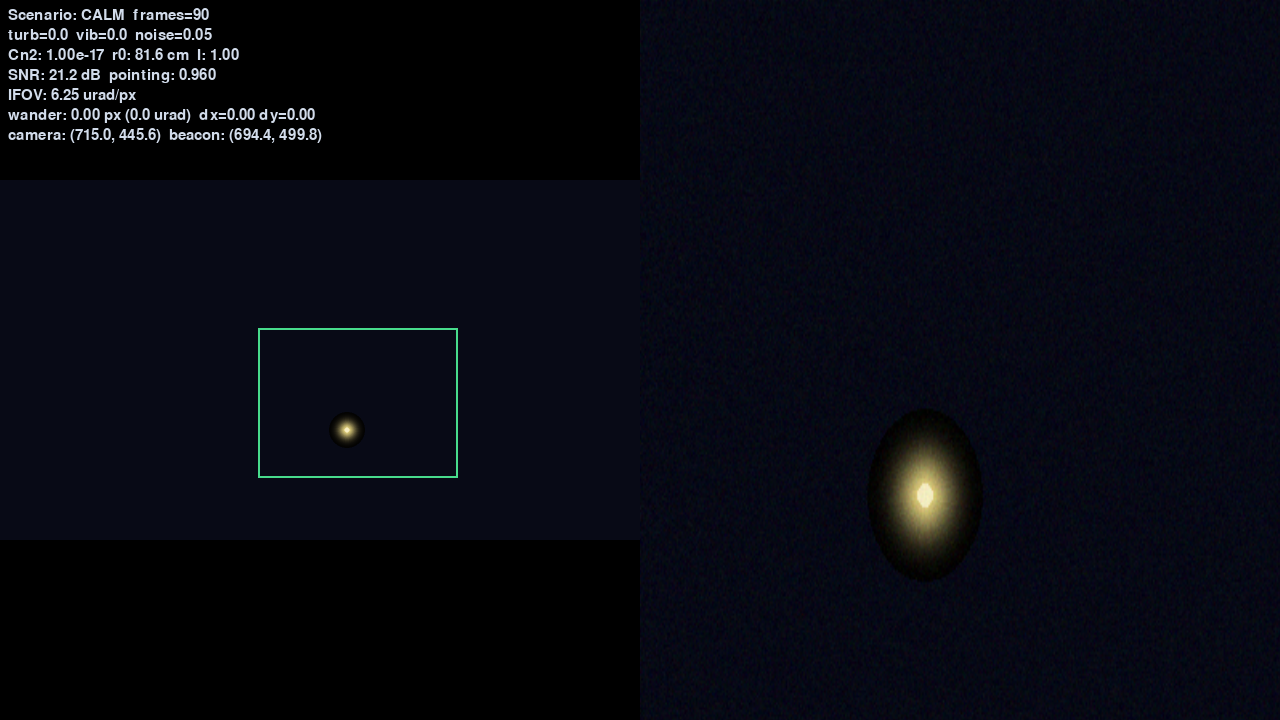
\includegraphics[width=\linewidth]{physics_calm.png}
  \caption{Calm}
  \label{fig:calm}
\end{subfigure}
\hfill
\begin{subfigure}{0.46\textwidth}
  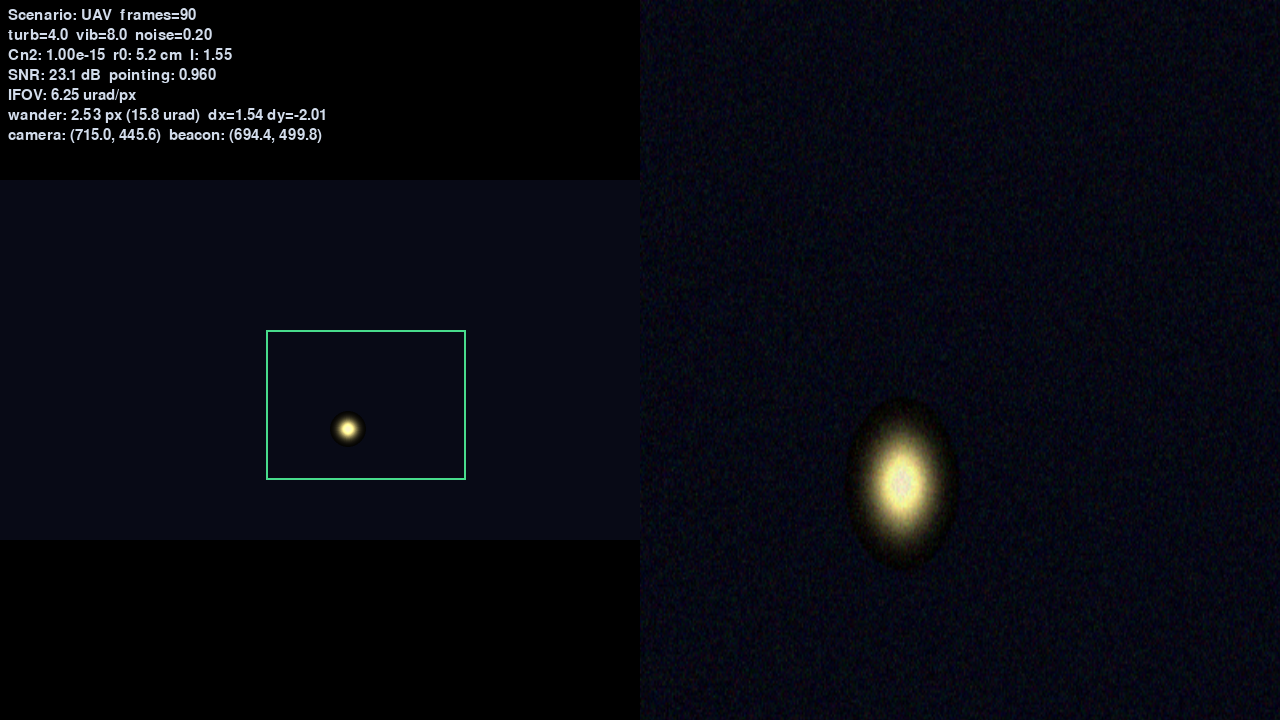
\includegraphics[width=\linewidth]{physics_uav.png}
  \caption{UAV}
  \label{fig:uav}
\end{subfigure}

\vspace{0.35em}
\begin{subfigure}{0.46\textwidth}
  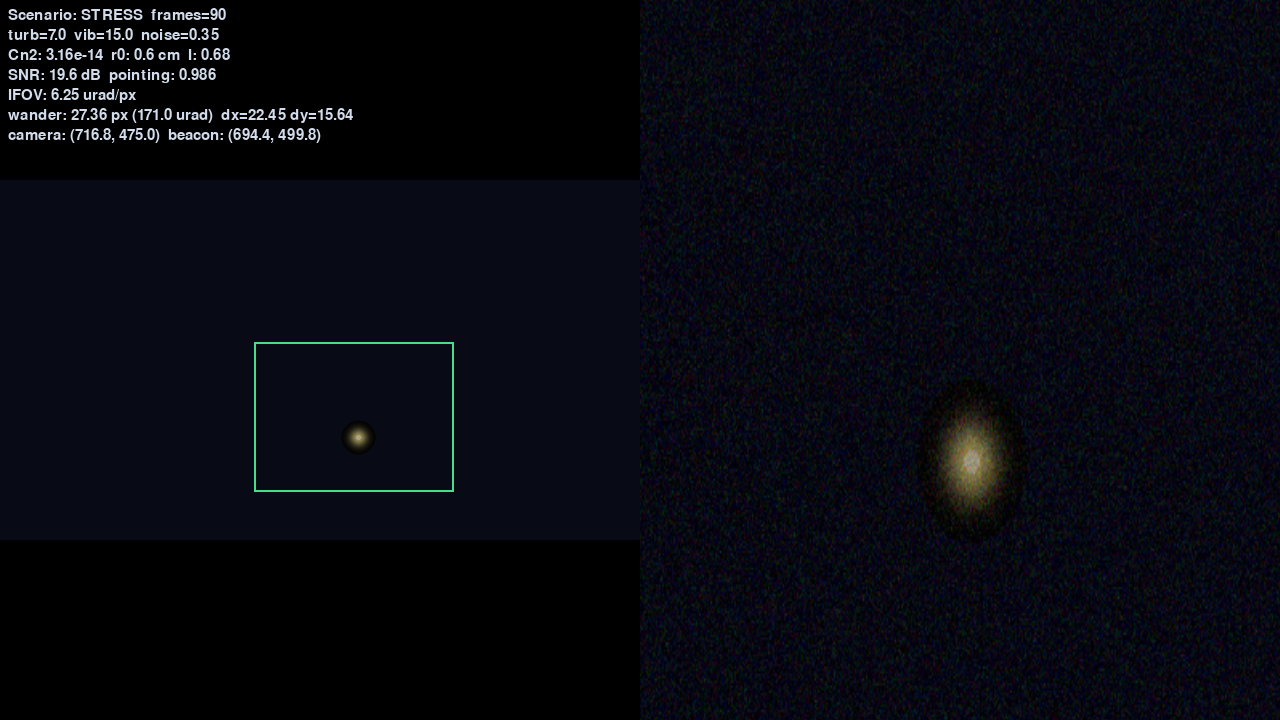
\includegraphics[width=\linewidth]{physics_stress.png}
  \caption{Stress}
  \label{fig:stress}
\end{subfigure}
\hfill
\begin{subfigure}{0.46\textwidth}
  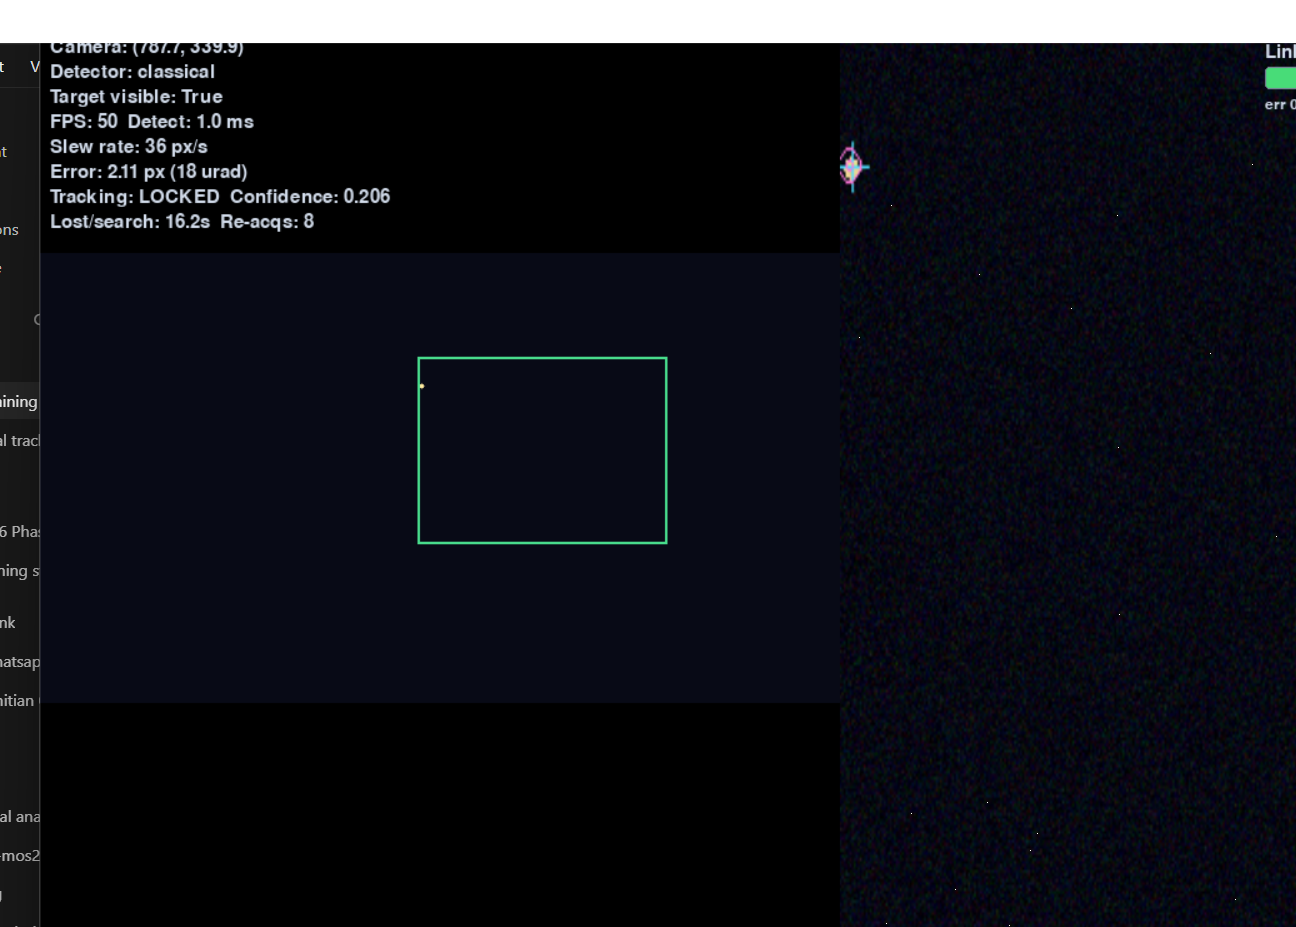
\includegraphics[width=\linewidth]{reacquire.png}
  \caption{Re-acquisition after loss}
  \label{fig:reacq}
\end{subfigure}
\caption{Live simulator captures (overview + camera FOV + HUD).}
\end{figure}

\begin{figure}[H]
\centering
\begin{subfigure}{0.42\textwidth}
  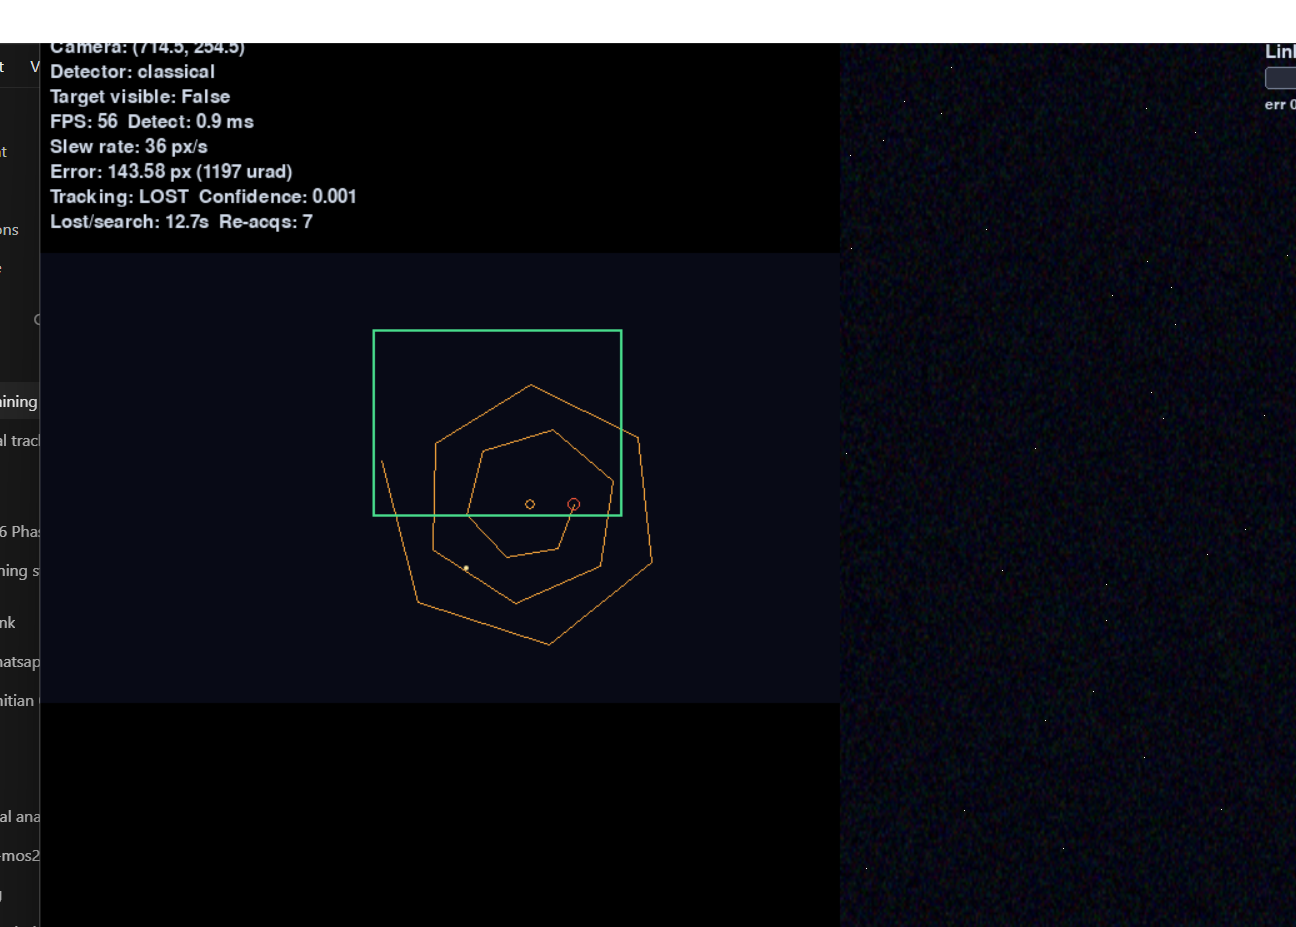
\includegraphics[width=\linewidth]{uav_locked.png}
  \caption{UAV locked tracking}
\end{subfigure}
\hfill
\begin{subfigure}{0.42\textwidth}
  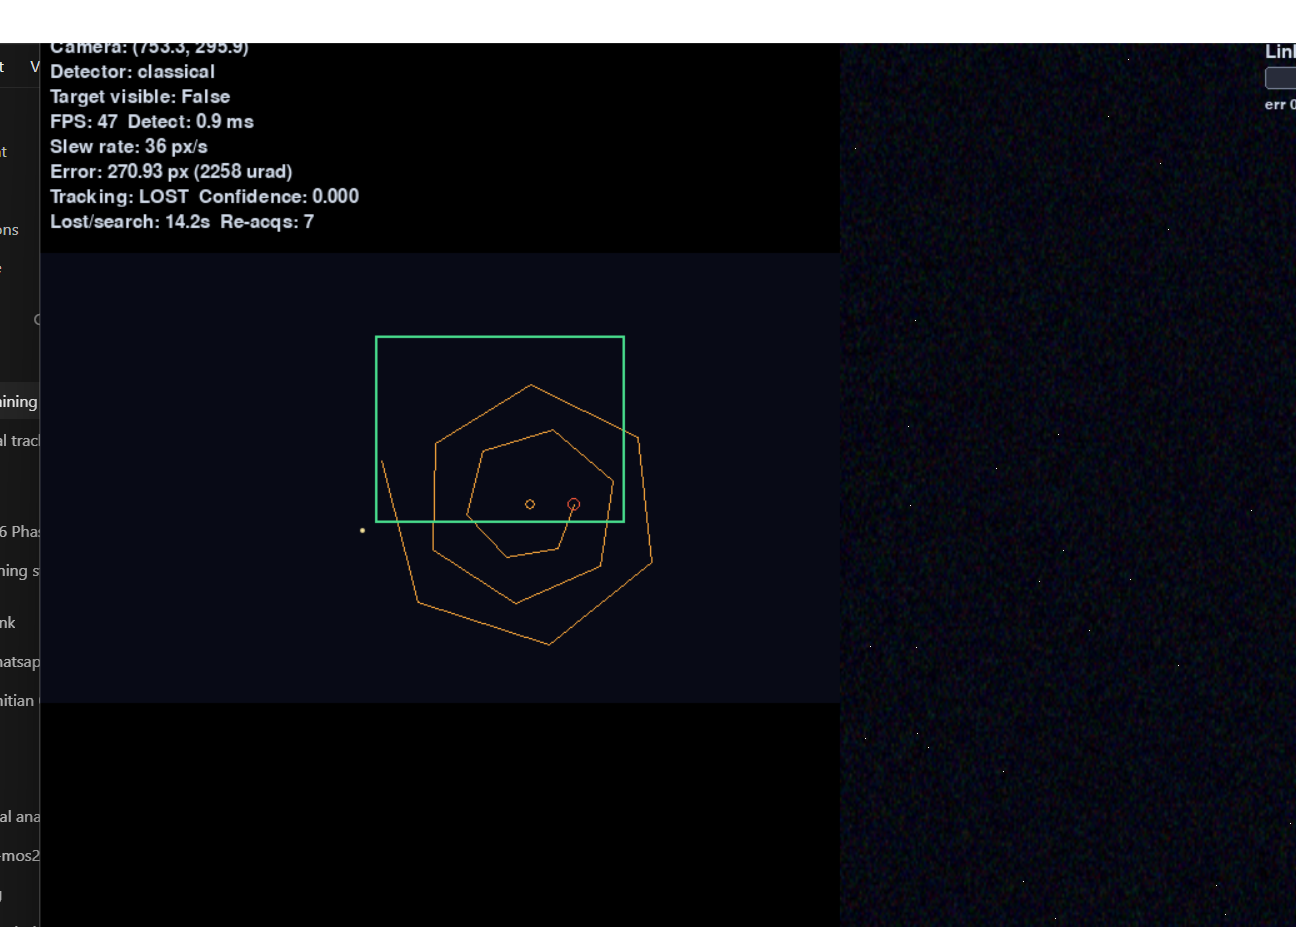
\includegraphics[width=\linewidth]{after_blind.png}
  \caption{After forced detector blind}
\end{subfigure}
\caption{Additional operational captures used in demos and reports.}
\label{fig:ops}
\end{figure}

\subsection{Matched-seed Classical vs AI matrix}
\begin{table}[H]
\centering
\caption{Scenario matrix (matched seed; mean error largely slew-lag limited)}
\label{tab:matrix}
\small
\begin{tabular}{@{}lccccc@{}}
\toprule
Scenario & C err & AI err & C lock & AI lock & Reacq C/AI \\
\midrule
Calm & 35.5\,px & 35.5\,px & 100\% & 100\% & 1 / 1 \\
UAV & 35.6\,px & 35.6\,px & 97.7\% & \textbf{100\%} & 1 / 1 \\
Stress & 35.1\,px & 36.1\,px & 95.5\% & 95.5\% & 2 / \textbf{1} \\
\bottomrule
\end{tabular}
\end{table}
\textbf{Interpretation.}
AI (hybrid) improves lock stability under UAV and reduces re-acquisitions under Stress.
Mean pixel error alone does not cleanly separate detectors because camera slew lag dominates the residual in physics mode ($\sim$35\,px $\approx$ $219\,\mu\mathrm{rad}$ at $6.25\,\mu\mathrm{rad/px}$).

\subsection{Acquisition Monte Carlo}
\begin{table}[H]
\centering
\caption{Time-to-lock Monte Carlo vs ESTOL-inspired 60\,s bound}
\label{tab:mc}
\begin{tabular}{@{}lcccc@{}}
\toprule
Scenario & Trials & Pass $<$60\,s & Median $T_{\mathrm{acq}}$ & p95 \\
\midrule
UAV & 40 & 40/40 & 0.82\,s & 0.85\,s \\
Stress & 40 & 40/40 & 0.97\,s & 1.0\,s \\
\bottomrule
\end{tabular}
\end{table}

\subsection{Benchmark-2 sample (PTZ bypass)}
On a synthetic full-frame noisy beacon MP4 with ground truth, Classical offline scoring achieved approximately \textbf{0.78\,px average centroid error} and \textbf{0.86\,px RMSE} with PTZ bypassed---well inside the suggested $\le10\,\mathrm{px}$ tracking-error class for that offline path.
This is the high-weight evaluation path when judges provide external video; closed-loop physics-mode mean error should not be conflated with Benchmark-2 centroid scoring.

\subsection{Discussion}
Performance should be judged primarily on lock retention, acquisition/re-acquisition timing, and reproducible logs.
Physics-mode mean error near 35\,px is a control-bandwidth effect, not necessarily a detection failure.
PS-profile geometry and higher °/s slew improve the prospect of meeting the Parameters-table $\le10\,\mathrm{px}$ guidance in closed-loop tests.
Link Readiness and Fine handoff are evaluated qualitatively in demos (readiness rises under lock + SNR; Fine engages with hysteresis) rather than as a BER certificate.

\subsection{Deliverables checklist}
All SIH submission deliverables are traced with status in Table~\ref{tab:evaldeliver}.
Mandatory items are \Done; the only \Partial\ item is optional demo-video length (a working demo MP4 already exists).

%% ============================================================
\section{Future Improvements}
%% ============================================================

\begin{enumerate}
  \item Lengthen the optional demo video to a full 3--5\,minutes with narration covering Calm $\rightarrow$ UAV $\rightarrow$ Stress $\rightarrow$ blind $\rightarrow$ Fine handoff.
  \item Ship a pre-built standalone executable package alongside the PyInstaller script.
  \item On-sky / real-camera fine-tuning of YOLO weights beyond synthetic data.
  \item Longer Monte Carlo campaigns with confidence intervals and spiral-vs-raster A/B under matched seeds.
  \item Optional offline phase-screen research mode while keeping the real-time statistical channel for demos.
  \item Hardware-in-the-loop bridge: stream real camera frames into the same detect--track API used by Benchmark-2.
  \item Closed-loop slew / prediction tuning in physics mode to shrink the $\sim$35\,px lag residual without destabilizing Stress re-acquisition.
\end{enumerate}

%% ============================================================
\section{Conclusion}
%% ============================================================

BeamLock delivers an AI-assisted virtual coarse PAT system for SIH26169 and \textbf{satisfies every mandatory expected-solution prerequisite} in the official problem statement, as shown in Section~\ref{sec:compliance} (Tables~\ref{tab:prereq}--\ref{tab:evaldeliver}).
Parameters-table geometry and controls are covered via the PS compliance profile; Evaluation Stages~1--2 tooling (including Benchmark-2 PTZ bypass) is ready; documentation deliverables are complete.
Beyond the written minima, BeamLock adds a physics channel, Link Readiness Fine handoff, hybrid AI fusion, and Monte Carlo acquisition evidence.
Verified results show hybrid AI improving UAV lock retention and reducing Stress re-acquisitions, sub-second median acquisition under Monte Carlo, and sub-pixel offline Benchmark-2 centroid error with PTZ bypass.
The project is positioned as a credible, reproducible software sandbox for PAT algorithm development under ISRO/DoS problem framing.

%% ============================================================
\section*{References}
%% ============================================================
\begin{enumerate}[leftmargin=1.6em,itemsep=0.3em]
  \item SDA Optical Communications Terminal (OCT) Standard --- PAT stage definitions.
  \item ESA ESTOL air interface --- acquisition-time guidance ($T_{\mathrm{acq}}<60\,\mathrm{s}$ class).
  \item ESA IZN-1 optical ground station materials --- acquisition FOV class.
  \item L.~C.~Andrews and R.~L.~Phillips, \emph{Laser Beam Propagation through Random Media}.
  \item M.~Kysel\'{a}k et al., ``Optimal Scanning Pattern for Initial Free-Space Optical-Link Alignment,'' \emph{Photonics}, 11(6):540, 2024.
  \item E.~Kohantorabi and M.~A.~Amirabadi, ``Design and hardware implementation of a robust deep vision-based FSO-PAT system,'' \emph{Applied Optics}.
  \item D.~Shivkant, S.~Jain, R.~K.~Ramakrishnan, ``Probabilistic Link Budget Analysis for LEO Satellites in the Optical Regime,'' arXiv:2507.20908.
  \item Smart India Hackathon Problem Statement SIH26169 (DoS/ISRO), Parameters and Evaluation tables.
\end{enumerate}

\vspace{1.0em}
\noindent\textit{End of SIH Technical Report --- BeamLock / Team Cadets.}

\end{document}
